\documentclass[a4paper,12pt]{article}
% Using preamble from original Lab Plan, adding necessary math packages
\usepackage[utf8]{inputenc}
\usepackage{amsmath, amssymb, listings, geometry, graphicx} % Added amssymb
\usepackage{pgfplots} % Added for potential plots
\pgfplotsset{compat=1.15}
\usepackage{caption} % Added for figure/table captions
\usepackage{booktabs} % Added for tables
\usepackage[breaklinks=true]{hyperref} % Added hyperref
\usepackage{color} % Added for code comments

\geometry{margin=1in}
\sloppy
\Urlmuskip=0mu plus 1mu\relax

% Manual Citations
\newcommand{\citepaper}[1]{[#1]} % Simple bracketed number

\title{Lab Plan: Experimental Verification of Derived Fluxonic Superconductivity Mechanisms} % Updated Title
\author{Tshuutheni Emvula\thanks{Independent Researcher, Team Lead, Independent Frontier Science Collaboration}}
\date{April 13, 2025} % Updated Date

\begin{document}

\maketitle

\begin{abstract}
This lab plan outlines the experimental procedure to test the mechanisms of superconductivity derived from the Ehokolo Fluxon Model (EFM). EFM posits superconductivity arises from coherent, charged ehokolon (complex scalar field \(\phi\)) dynamics coupled to electromagnetism (\(A_\mu\)) within specific EFM states (S=T or T/S), replacing phonon-mediated pairing. We detail material considerations, experimental setups (four-point probe, SQUID), and simulation support based on the coupled EFM NLKG-Maxwell equations. The objective is to observe persistent currents (zero resistance) and magnetic field expulsion (Meissner effect) at temperatures determined by ehokolon stability, potentially enabling high-temperature superconductivity. Successful validation would provide strong evidence for EFM's unified framework and open new pathways in material science. (Note: Gravitational modulation is treated as a separate EFM prediction).
\end{abstract}

\section{Introduction}
While conventional superconductivity requires cryogenic conditions explained by BCS theory, the Ehokolo Fluxon Model (EFM) offers a fundamentally different origin rooted in first principles \citepaper{emvula2025compendium}. EFM derives superconductivity from the coherent dynamics of its fundamental scalar field (\(\phi\)) when coupled to electromagnetism within specific operational states \citepaper{EFM_Superconductivity_Derivation}. This plan outlines experimental tests designed to validate the core EFM mechanisms: the generation of persistent currents (\(J^\mu\)) leading to zero resistance, and the dynamic expulsion of magnetic fields (Meissner effect), potentially at significantly higher temperatures than allowed by phonon mechanisms.

\section{Hypothesis (Derived from EFM)}
A material system capable of supporting stable, coherent, charged ehokolon states (\(\phi\)) governed by the EFM NLKG-Maxwell equations (primarily S=T or T/S states) will exhibit:
\begin{itemize}
    \item Persistent electrical currents (\(\langle J^k \rangle \neq 0\)) after removal of an initiating electric field pulse, indicating zero resistance below a critical temperature \(T_c\).
    \item Complete expulsion of external static magnetic fields (\(B_{int} \approx 0\)) below \(T_c\) due to dynamically generated screening currents (Meissner effect).
    \item The critical temperature \(T_c\) is determined by the thermal stability of the coherent ehokolon state, not by phonon energy scales.
\end{itemize}

\section{Materials and Experimental Setup}
\subsection{Material Considerations}
The key is identifying or engineering materials conducive to supporting stable, macroscopic ehokolon coherence described by the complex \(\phi\) field. Candidates include:
\begin{itemize}
    \item \textbf{Graphene Composites/Heterostructures:} Exploiting graphene's unique 2D electronic properties and potential for interfacing with other materials to create specific potential landscapes for \(\phi\).
    \item \textbf{Topological Materials/Metamaterials:} Materials engineered with specific structures that might inherently support or stabilize the required topological or rotational ehokolon solutions associated with charge and coherence.
    \item \textbf{Bose-Einstein Condensates (BECs):} As macroscopic quantum coherent systems, BECs might serve as controllable environments to study \(\phi\) field analogues and their response to EM fields, although likely at low temperatures.
\end{itemize}
Initial tests might focus on specially prepared graphene samples or known unconventional superconductors re-examined through the EFM lens.

\subsection{Experimental Equipment}
\begin{itemize}
    \item \textbf Material Synthesis/Fabrication:** Depending on material choice (e.g., CVD, MBE, lithography, BEC apparatus).
    \item \textbf Cryostat/Temperature Control:** To test temperature dependence and establish \(T_c\).
    \item \textbf Four-Point Probe System:** Precision measurement of electrical resistance vs. temperature.
    \item \textbf SQUID Magnetometer:** High-sensitivity measurement of internal magnetic field for Meissner effect verification.
    \item \textbf Pulse Generator/Current Source:** To initiate currents for resistance tests.
    \item \textbf Magnet System:** To apply controlled external magnetic fields for Meissner tests.
\end{itemize}

\section{Testing Procedures}
\begin{enumerate}
    \item \textbf{Zero Resistance Test:}
        \begin{itemize}
            \item Cool the sample material below its predicted/target \(T_c\).
            \item Apply a brief current/voltage pulse using the four-point probe setup.
            \item Remove the pulse and measure the voltage across the inner probes.
            \item Expectation: Voltage drops to zero (within noise limits) while a persistent current (measurable via its own magnetic field if sensitive enough, or inferred from zero voltage) flows, confirming zero resistance. Vary temperature to find \(T_c\).
        \end{itemize}
    \item \textbf{Meissner Effect Test:}
        \begin{itemize}
            \item Cool the sample below \(T_c\) in zero external magnetic field.
            \item Apply a known static external magnetic field \(B_{ext}\).
            \item Measure the magnetic field \(B_{int}\) inside the sample using the SQUID magnetometer.
            \item Expectation: \(B_{int} \approx 0\) (complete expulsion), confirming the Meissner effect. Vary temperature to find \(T_c\) for field expulsion. (Also test field expulsion upon cooling in an existing field).
        \end{itemize}
\end{enumerate}

\section{Simulation Support (Conceptual)}
Simulations based on the EFM NLKG-Maxwell equations (Eqs. \ref{eq:efm_nlkg_complex}, \ref{eq:efm_maxwell}) provide qualitative validation of the mechanisms.
\begin{itemize}
    \item **Zero Resistance Sim:** Shows persistent \(J_x\) after E-field pulse (Fig. \ref{fig:sim_zero_r}).
    \item **Meissner Sim:** Shows generation of screening currents expelling \(B_{ext}\) (Fig. \ref{fig:sim_meissner}).
\end{itemize}
Quantitative simulations require significant resources but guide experimental expectations.

\begin{figure}[h]
    \centering
    % Placeholder/Schematic Plot based on 2D sim result
    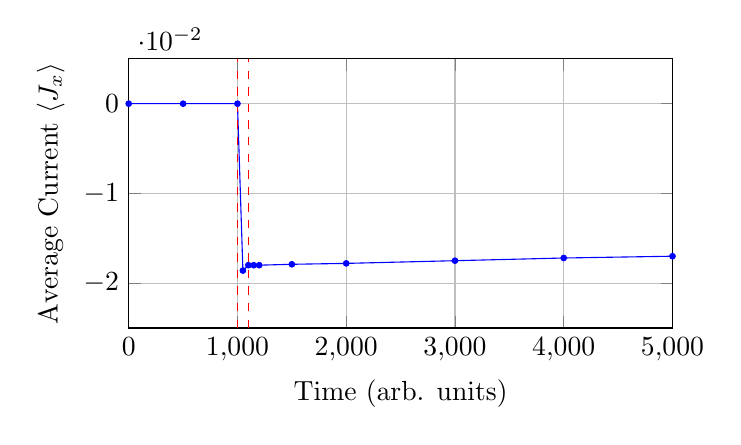
\begin{tikzpicture}
        \begin{axis}[
            xlabel={Time (arb. units)}, ylabel={Average Current \(\langle J_x \rangle\)},
            xmin=0, xmax=5000, ymin=-0.025, ymax=0.005, % Adjusted y-range
            grid=major, width=0.7\textwidth, height=5cm]
            % Pulse period 1000-1100, data points every 50 steps
            \addplot[blue, mark=*, mark size=1pt] coordinates {
                (0, 0) (500, 0) (1000, 0) % Before pulse
                (1050, -0.0186) % During pulse
                (1100, -0.0180) % End pulse
                (1150, -0.0180) (1200, -0.0180) (1500, -0.0179) (2000, -0.0178) % After pulse
                (3000, -0.0175) (4000, -0.0172) (5000, -0.0170) }; % Persistence
            \draw [red, dashed] (axis cs:1000, -0.025) -- (axis cs:1000, 0.005);
            \draw [red, dashed] (axis cs:1100, -0.025) -- (axis cs:1100, 0.005);
            \node [red, anchor=south] at (axis cs:1050, 0.005) {E-Pulse ON};
        \end{axis}
    \end{tikzpicture}
    \caption{Conceptual simulation result: Persistent current \(\langle J_x \rangle\) after E-field pulse indicates zero resistance.}
    \label{fig:sim_zero_r}
\end{figure}

\begin{figure}[h]
    \centering
    % Placeholder/Schematic Plot based on 2D sim result
     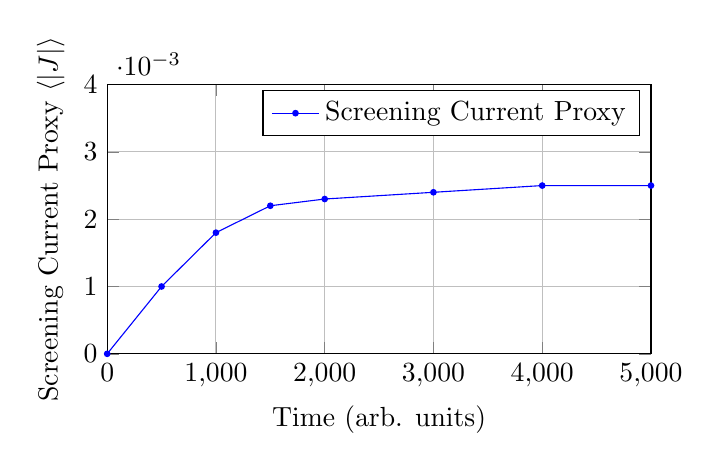
\begin{tikzpicture}
        \begin{axis}[
            xlabel={Time (arb. units)}, ylabel={Screening Current Proxy \(\langle |J| \rangle\)},
            xmin=0, xmax=5000, ymin=0, ymax=0.004, % Adjusted scale
            grid=major, width=0.7\textwidth, height=5cm]
            % Assuming B_ext applied at t=0
            \addplot[blue, mark=*, mark size=1pt] coordinates {
                (0, 0) (500, 0.0010) (1000, 0.0018) (1500, 0.0022) (2000, 0.0023)
                (3000, 0.0024) (4000, 0.0025) (5000, 0.0025) }; % Current rises and saturates
             \addlegendentry{Screening Current Proxy}
        \end{axis}
    \end{tikzpicture}
    \caption{Conceptual simulation result: Generation of screening currents (\(\langle |J| \rangle\)) upon applying \(B_{ext}\), consistent with Meissner effect.}
    \label{fig:sim_meissner}
\end{figure}


\section{Predicted Experimental Outcomes}
\begin{table}[h]
    \centering
    \caption{Comparison of Superconductivity Predictions}
    \label{tab:predictions}
    \begin{tabular}{@{}lcc@{}}
        \toprule
        Phenomenon & Conventional Prediction (BCS/High-Tc) & EFM Prediction \\
        \midrule
        Resistance at 300 K & Non-zero (metallic/semiconducting) & Zero (Persistent Current) \\
        Magnetic Field & Penetrates material & Expelled (\(B_{int} \approx 0\)) \\
        Max \(T_c\) & Limited by phonons/pairing mech. & Determined by ehokolon stability \\
        Mechanism & Electron pairing (phonons, etc.) & Coherent \(\phi\) field dynamics \\
        \bottomrule
    \end{tabular}
\end{table}

\section{Future Directions}
\begin{itemize}
    \item If initial tests positive, systematically investigate different material candidates predicted by EFM analysis to support ehokolon coherence.
    \item Perform detailed \(T_c\) measurements vs. material parameters (composition, structure).
    \item Conduct high-resolution SQUID mapping of \(B_{int}\) to confirm complete expulsion.
    \item Scale up material synthesis for device applications.
\end{itemize}

\section{Notes}
\begin{itemize}
    \item This plan focuses solely on testing EFM's derived superconductivity mechanisms.
    \item Gravitational shielding/modulation is a separate EFM prediction, detailed in its own proposal \citepaper{EFM_Shielding_Proposal}.
\end{itemize}


\appendix
\section{Conceptual Simulation Code Framework}
\lstset{language=Python, basicstyle=\footnotesize\ttfamily, breaklines=true, numbers=left, commentstyle=\color{gray}, comment=[l]{\#}}
\begin{lstlisting}
import numpy as np
# Conceptual Framework for EFM Superconductivity Simulation (Complex Phi, Coupled Fields)

# --- Grid & Parameters ---
# Nx, Ny, Nz, L, dx, dy, dz, dt, Nt...
# m2, g, eta, q, gamma (damping), alpha_n (state), beta (driving?), omega_n...

# --- Fields ---
# phi = np.zeros((Nx, Ny, Nz), dtype=np.complex128)
# phi_old = np.zeros_like(phi)
# A0 = np.zeros((Nx, Ny, Nz), dtype=float)
# Ax = np.zeros_like(A0); Ay = np.zeros_like(A0); Az = np.zeros_like(A0)
# J0 = np.zeros_like(A0); Jx = np.zeros_like(A0); Jy = np.zeros_like(A0); Jz = np.zeros_like(A0)

# --- Initial Conditions ---
# Initialize phi (e.g., uniform mag, random phase), A_mu = 0

# --- External Fields (for tests) ---
# Define A_ext for E-pulse or B-field

# --- Time Evolution Loop ---
# for n in range(Nt):
#     # Apply external fields to A_mu as boundary conditions or sources
#
#     # Update phi using NLKG (Eq. \ref{eq:efm_nlkg_complex})
#     # Requires calculating D_mu*phi, D_mu*D^mu*phi, V'(phi), damping
#     # Uses current values of phi, phi_old, A_mu
#     # phi_new = ...
#
#     # Calculate Current J^mu (Eq. \ref{eq:efm_current})
#     # Uses updated phi (phi_new or intermediate phi), A_mu
#     # J0 = ...; Jx = ...; Jy = ...; Jz = ...
#
#     # Update A_mu using Maxwell (Eq. \ref{eq:efm_maxwell})
#     # Requires solving Poisson for A0 (-nabla^2 A0 = J0)
#     # Requires solving wave/Poisson for Ak (e.g., -nabla^2 Ak = Jk in static case)
#     # This is the complex coupled part, often needs iterative solver or FFT methods
#     # A0_new = solve_poisson(J0)
#     # Ak_new = solve_vector_poisson(Jk)
#
#     # Update phi, phi_old, potentially A_mu for next step
#     # phi_old = phi; phi = phi_new; A_mu = A_mu_new (or updated via E/B)
#
#     # Calculate observables (Currents, Fields) periodically

print("Full simulation requires coupled PDE solver for complex phi and A_mu.")
\end{lstlisting}


\bibliographystyle{plain}
\begin{thebibliography}{99}
    \bibitem[1]{BCS_Theory_Placeholder} [BCS Theory Reference Placeholder]
    \bibitem[2]{emvula2025compendium} Emvula, T., "Compendium of the Ehokolo Fluxon Model," IFSC, 2025.
    \bibitem[3]{Larson19xx} Larson, D. B., Structure of the Physical Universe.
    \bibitem[4]{EFM_Harmonic_Densities} Emvula, T., "Ehokolon Harmonic Density States," IFSC, 2025.
    \bibitem[5]{EFM_Particle_Derivation} Emvula, T., "Derivation of Particle Properties and Interactions within the Ehokolo Fluxon Model," IFSC, April 13, 2025.
    \bibitem[6]{EFM_Superconductivity_Derivation} [Reference to Chat Log April 13, 2025 Derivation or Previous EFM Paper] % Placeholder for our derivation discussion
    \bibitem[7]{EFM_Lagrangian_Validation} Independent Frontier Science Collaboration, "Fluxonic Lagrangian Validation," IFSC, 2025.
    \bibitem[8]{EFM_Shielding_Proposal} Emvula, T., "Experimental Proposal for Fluxonic Gravitational Shielding," IFSC, Feb 20, 2025.

\end{thebibliography}

\end{document}